\documentclass{article}\usepackage[]{graphicx}\usepackage[]{xcolor}
% maxwidth is the original width if it is less than linewidth
% otherwise use linewidth (to make sure the graphics do not exceed the margin)
\makeatletter
\def\maxwidth{ %
  \ifdim\Gin@nat@width>\linewidth
    \linewidth
  \else
    \Gin@nat@width
  \fi
}
\makeatother

\definecolor{fgcolor}{rgb}{0.345, 0.345, 0.345}
\newcommand{\hlnum}[1]{\textcolor[rgb]{0.686,0.059,0.569}{#1}}%
\newcommand{\hlsng}[1]{\textcolor[rgb]{0.192,0.494,0.8}{#1}}%
\newcommand{\hlcom}[1]{\textcolor[rgb]{0.678,0.584,0.686}{\textit{#1}}}%
\newcommand{\hlopt}[1]{\textcolor[rgb]{0,0,0}{#1}}%
\newcommand{\hldef}[1]{\textcolor[rgb]{0.345,0.345,0.345}{#1}}%
\newcommand{\hlkwa}[1]{\textcolor[rgb]{0.161,0.373,0.58}{\textbf{#1}}}%
\newcommand{\hlkwb}[1]{\textcolor[rgb]{0.69,0.353,0.396}{#1}}%
\newcommand{\hlkwc}[1]{\textcolor[rgb]{0.333,0.667,0.333}{#1}}%
\newcommand{\hlkwd}[1]{\textcolor[rgb]{0.737,0.353,0.396}{\textbf{#1}}}%
\let\hlipl\hlkwb

\usepackage{framed}
\makeatletter
\newenvironment{kframe}{%
 \def\at@end@of@kframe{}%
 \ifinner\ifhmode%
  \def\at@end@of@kframe{\end{minipage}}%
  \begin{minipage}{\columnwidth}%
 \fi\fi%
 \def\FrameCommand##1{\hskip\@totalleftmargin \hskip-\fboxsep
 \colorbox{shadecolor}{##1}\hskip-\fboxsep
     % There is no \\@totalrightmargin, so:
     \hskip-\linewidth \hskip-\@totalleftmargin \hskip\columnwidth}%
 \MakeFramed {\advance\hsize-\width
   \@totalleftmargin\z@ \linewidth\hsize
   \@setminipage}}%
 {\par\unskip\endMakeFramed%
 \at@end@of@kframe}
\makeatother

\definecolor{shadecolor}{rgb}{.97, .97, .97}
\definecolor{messagecolor}{rgb}{0, 0, 0}
\definecolor{warningcolor}{rgb}{1, 0, 1}
\definecolor{errorcolor}{rgb}{1, 0, 0}
\newenvironment{knitrout}{}{} % an empty environment to be redefined in TeX

\usepackage{alltt}
\usepackage{graphicx}
\usepackage{geometry}
\geometry{
  a4paper,
  total={170mm,257mm},
  left=20mm,
  top=20mm
}

\title{Informe de Análisis de Datos}
\author{Ana G. Dos Santos F.}
\date{2024-07-24}
\IfFileExists{upquote.sty}{\usepackage{upquote}}{}
\begin{document}
\maketitle

\section*{Primeros pasos}

\begin{itemize}
\item Instalar una distribución de \LaTeX{}: tinytex
\item Instalar knitr si fuera necesario
\item cargar librerias necesarias 'here', 'readr', 'dplyr' y 'ggplot2'
\item Configurar globalmente los Chunk
\item Importar la BBDD Depurada
\item Instalar paquetes de \LaTeX{} mediante tinytex como por ejemplo 'graphicx'
\end{itemize}





\section{Requisitos del entregable}
\subsection{Deberá contener al menos 2 de los siguientes:}

\begin{itemize}
\item Un gráfico con los principales resultados.
\item Explicaciones que combinen resultados de R (insertados mediante código) con texto con formato.
\item Una tabla resumen con algunos indicadores.
\end{itemize}

\section{Introducción}
Este informe presenta el análisis de los datos depurados del conjunto de datos ESS9e03\_2-ESS10.

\section{Análisis de Datos}

\subsection{Visualización de Gráficos}


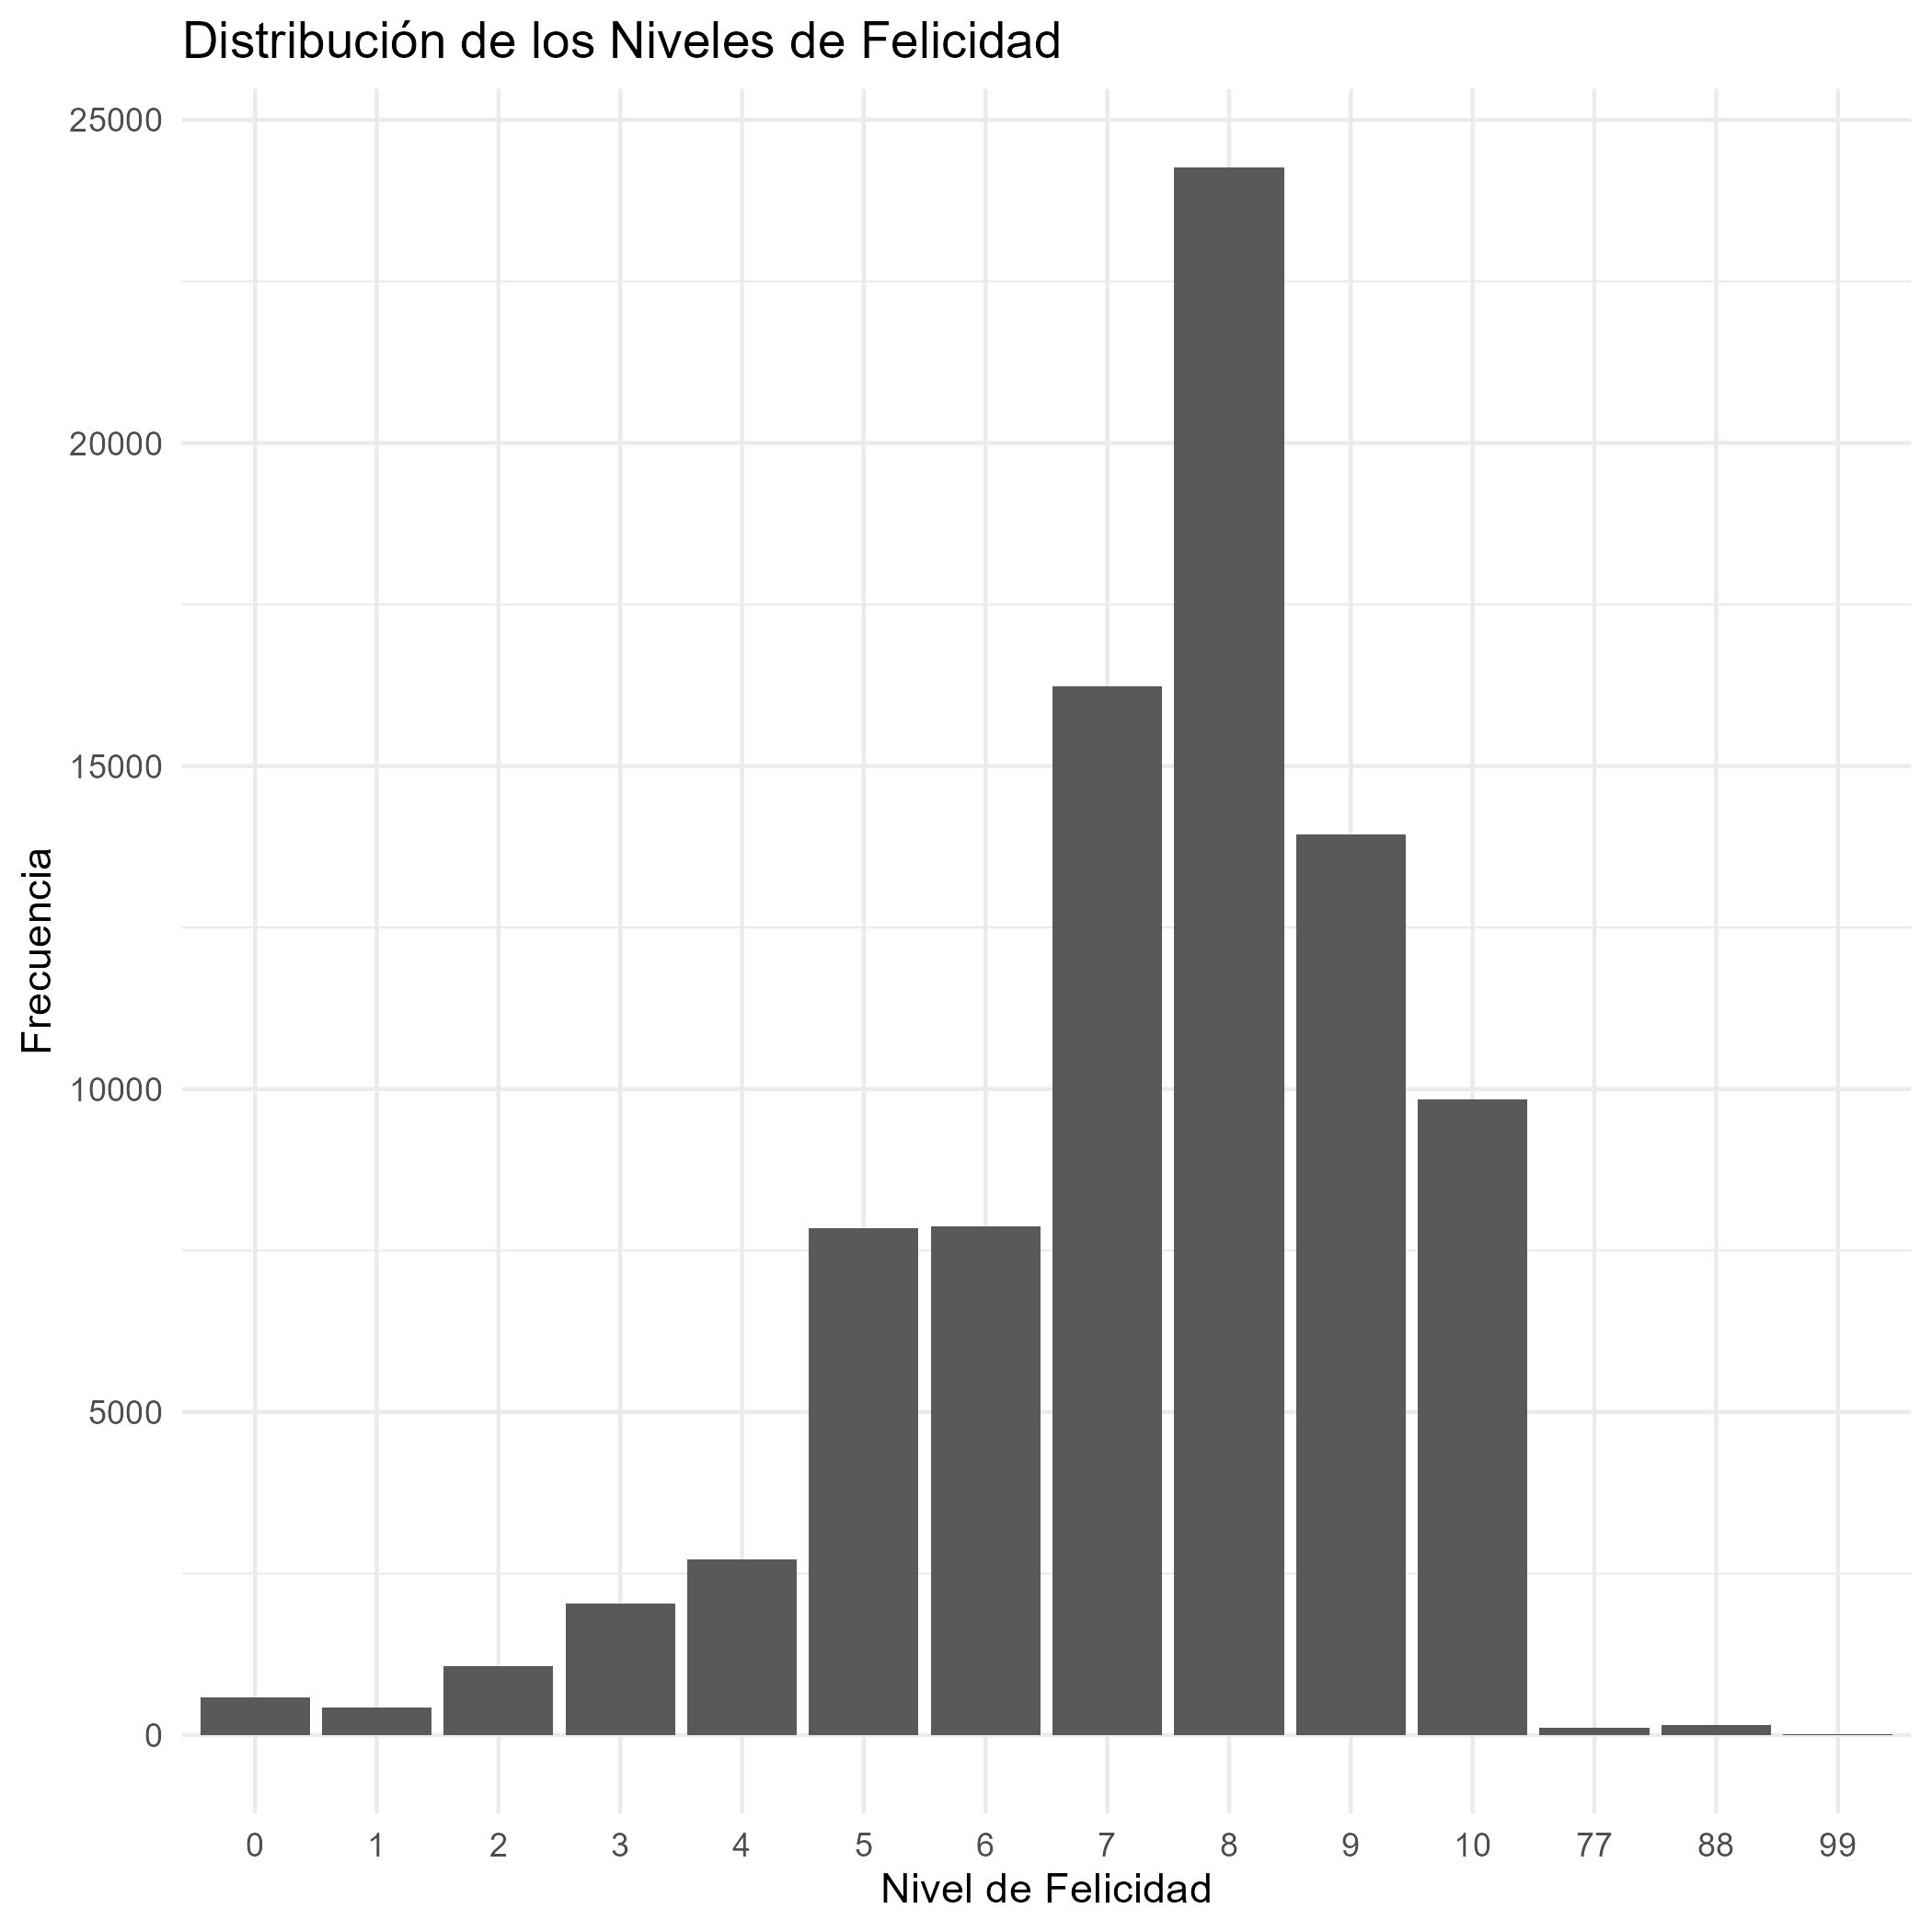
\includegraphics[width=\maxwidth]{distribucion_felicidad} 

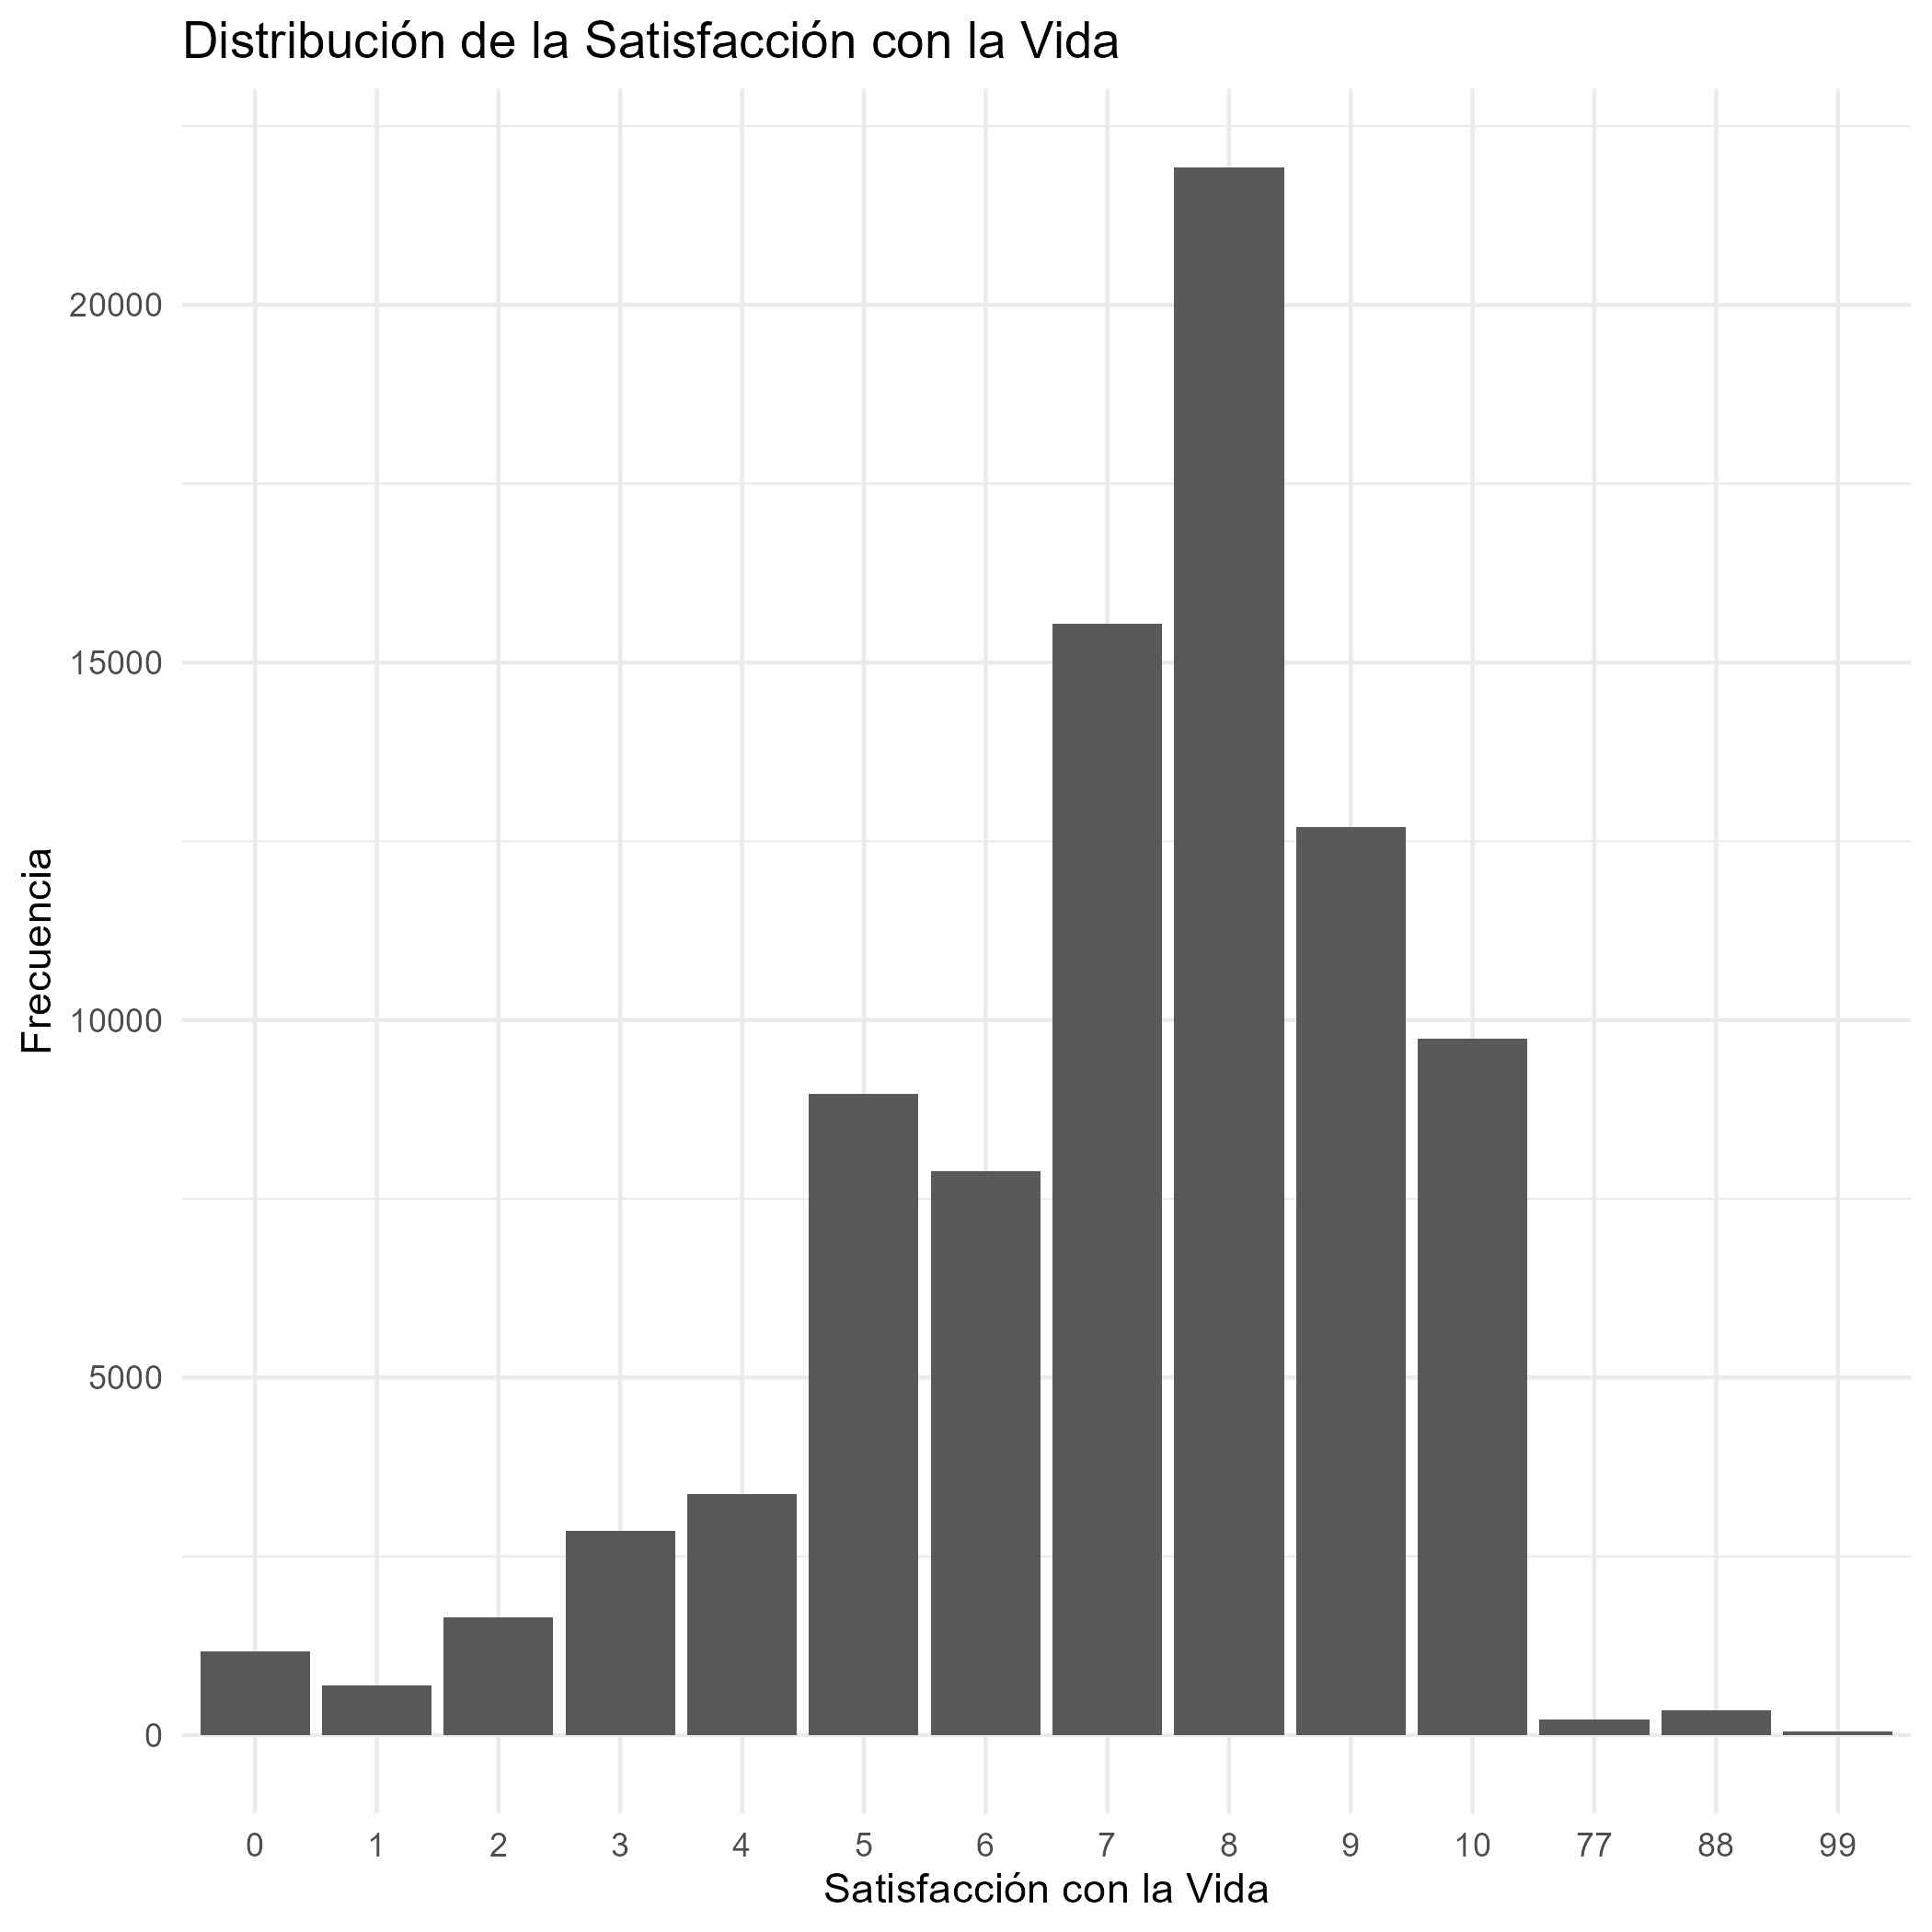
\includegraphics[width=\maxwidth]{distribucion_satisfaccion_vida} 

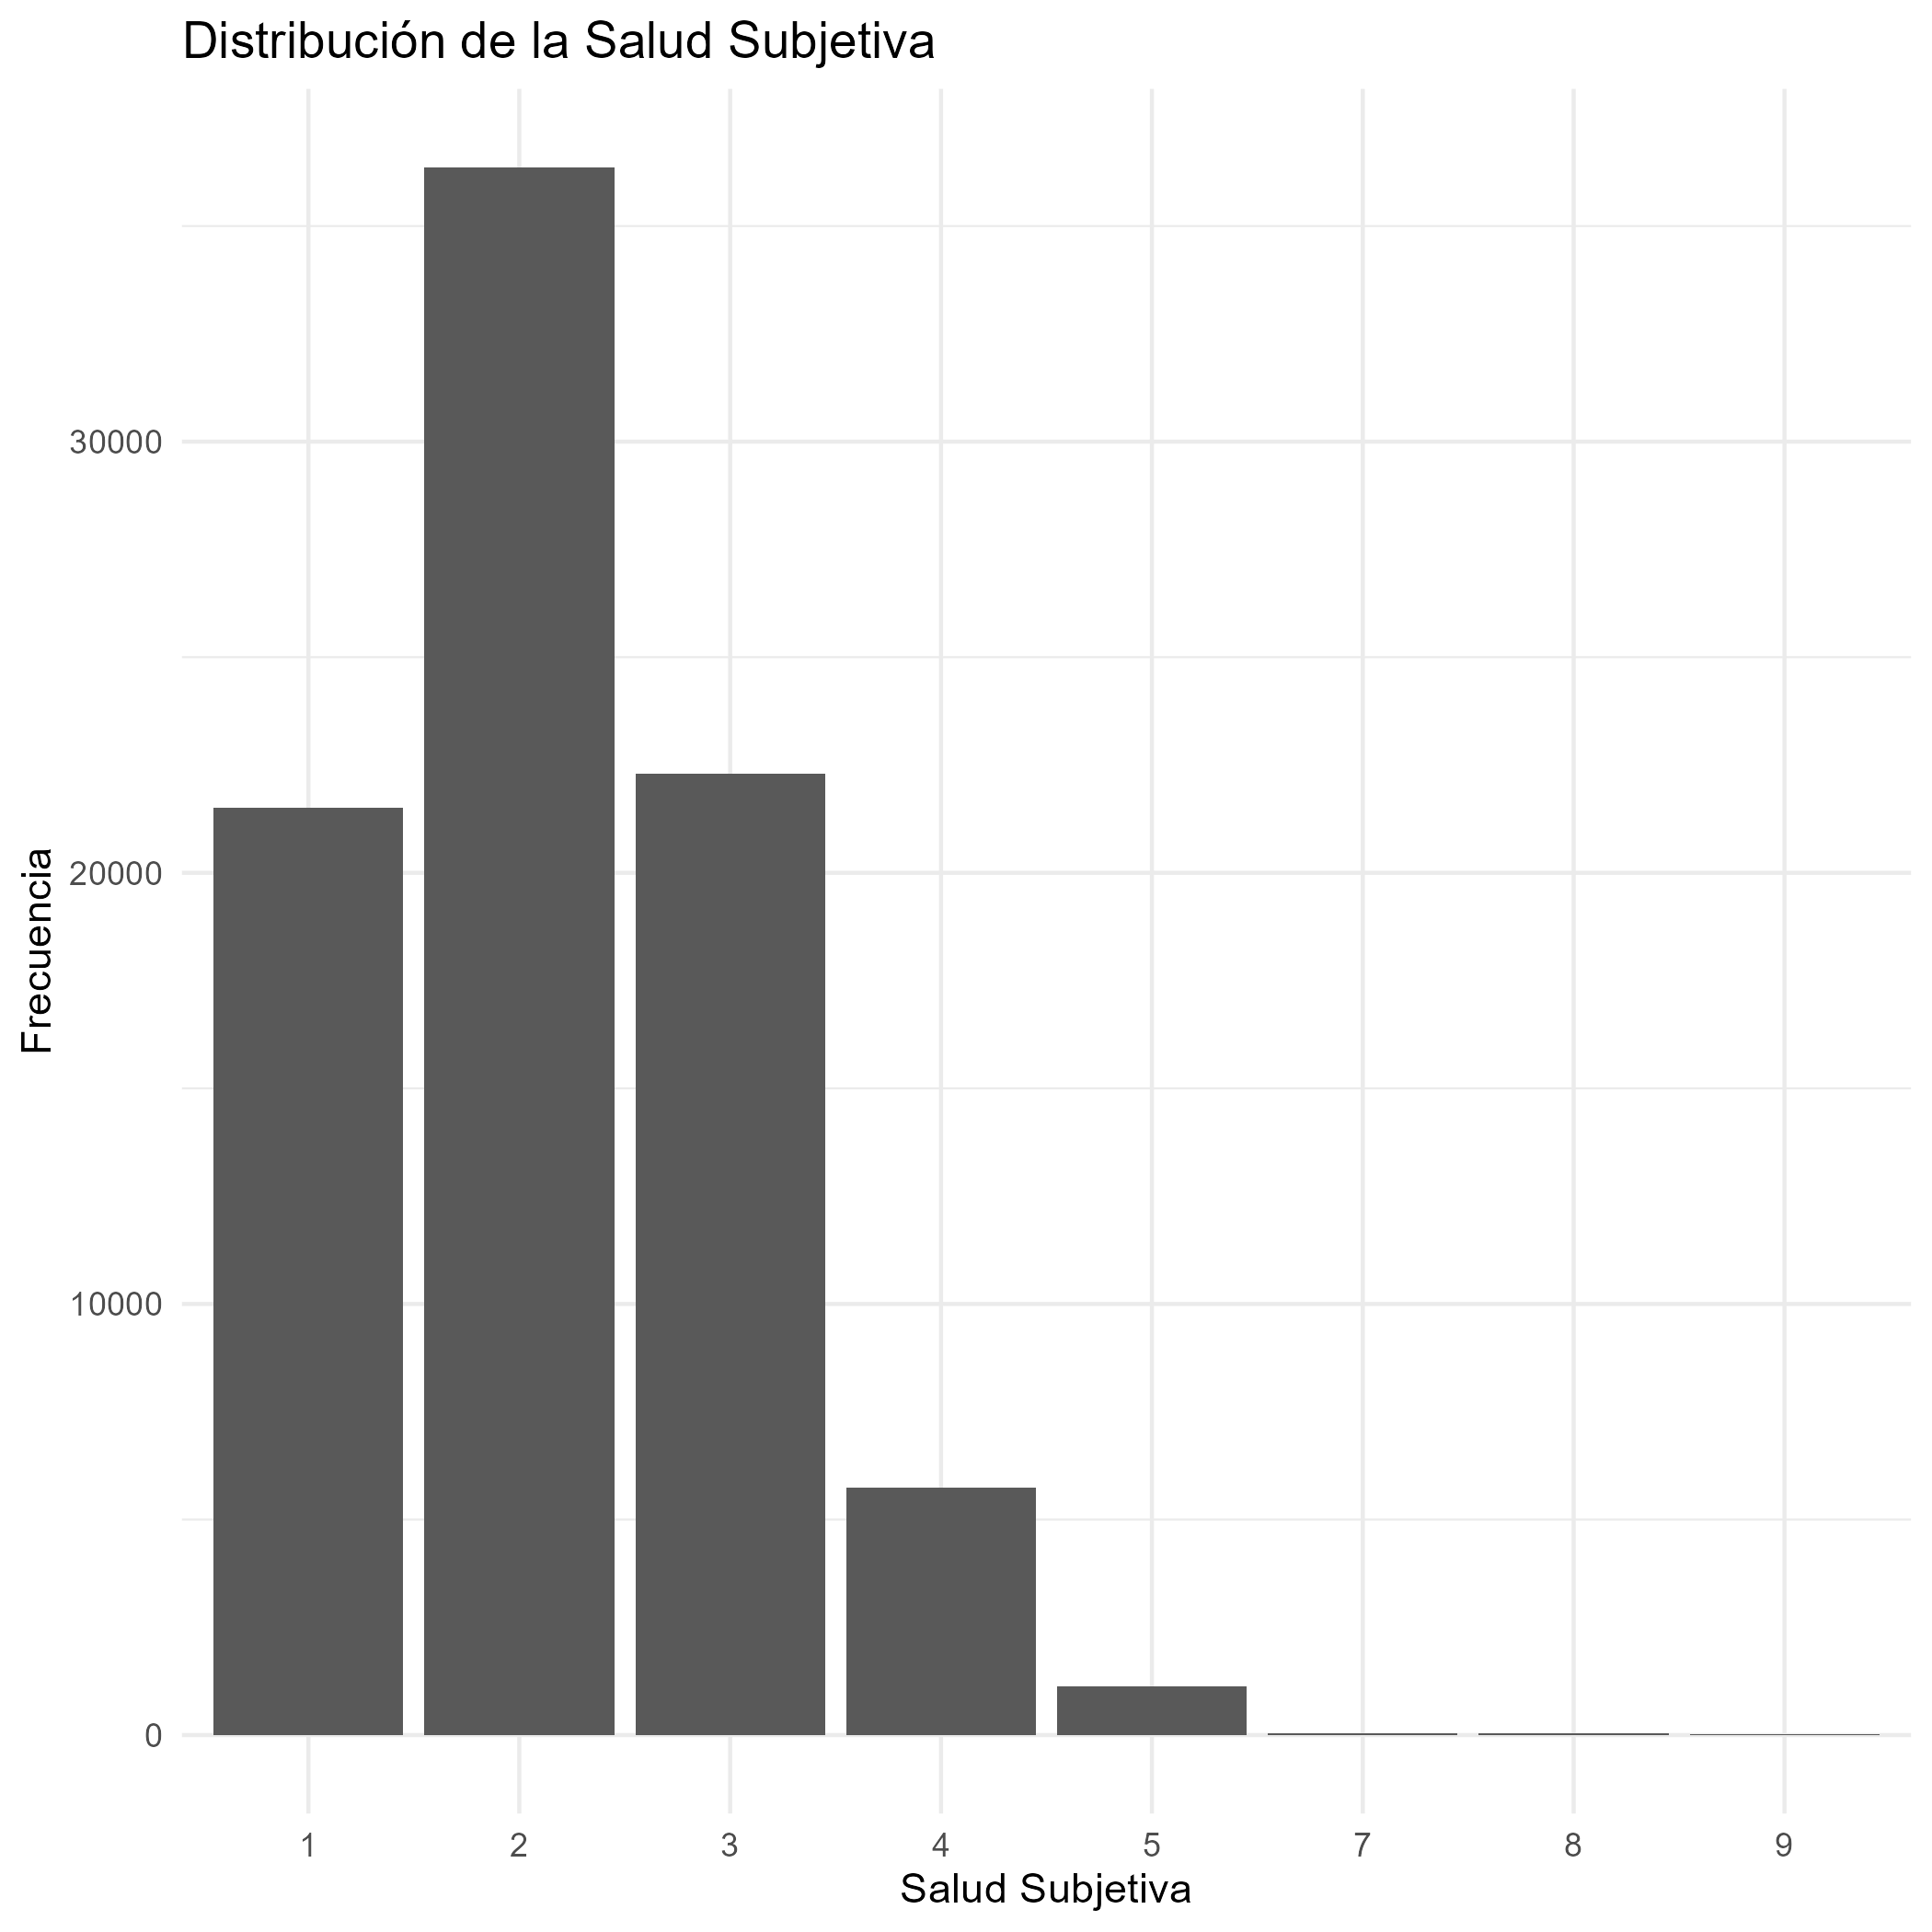
\includegraphics[width=\maxwidth]{distribucion_salud_subjetiva} 

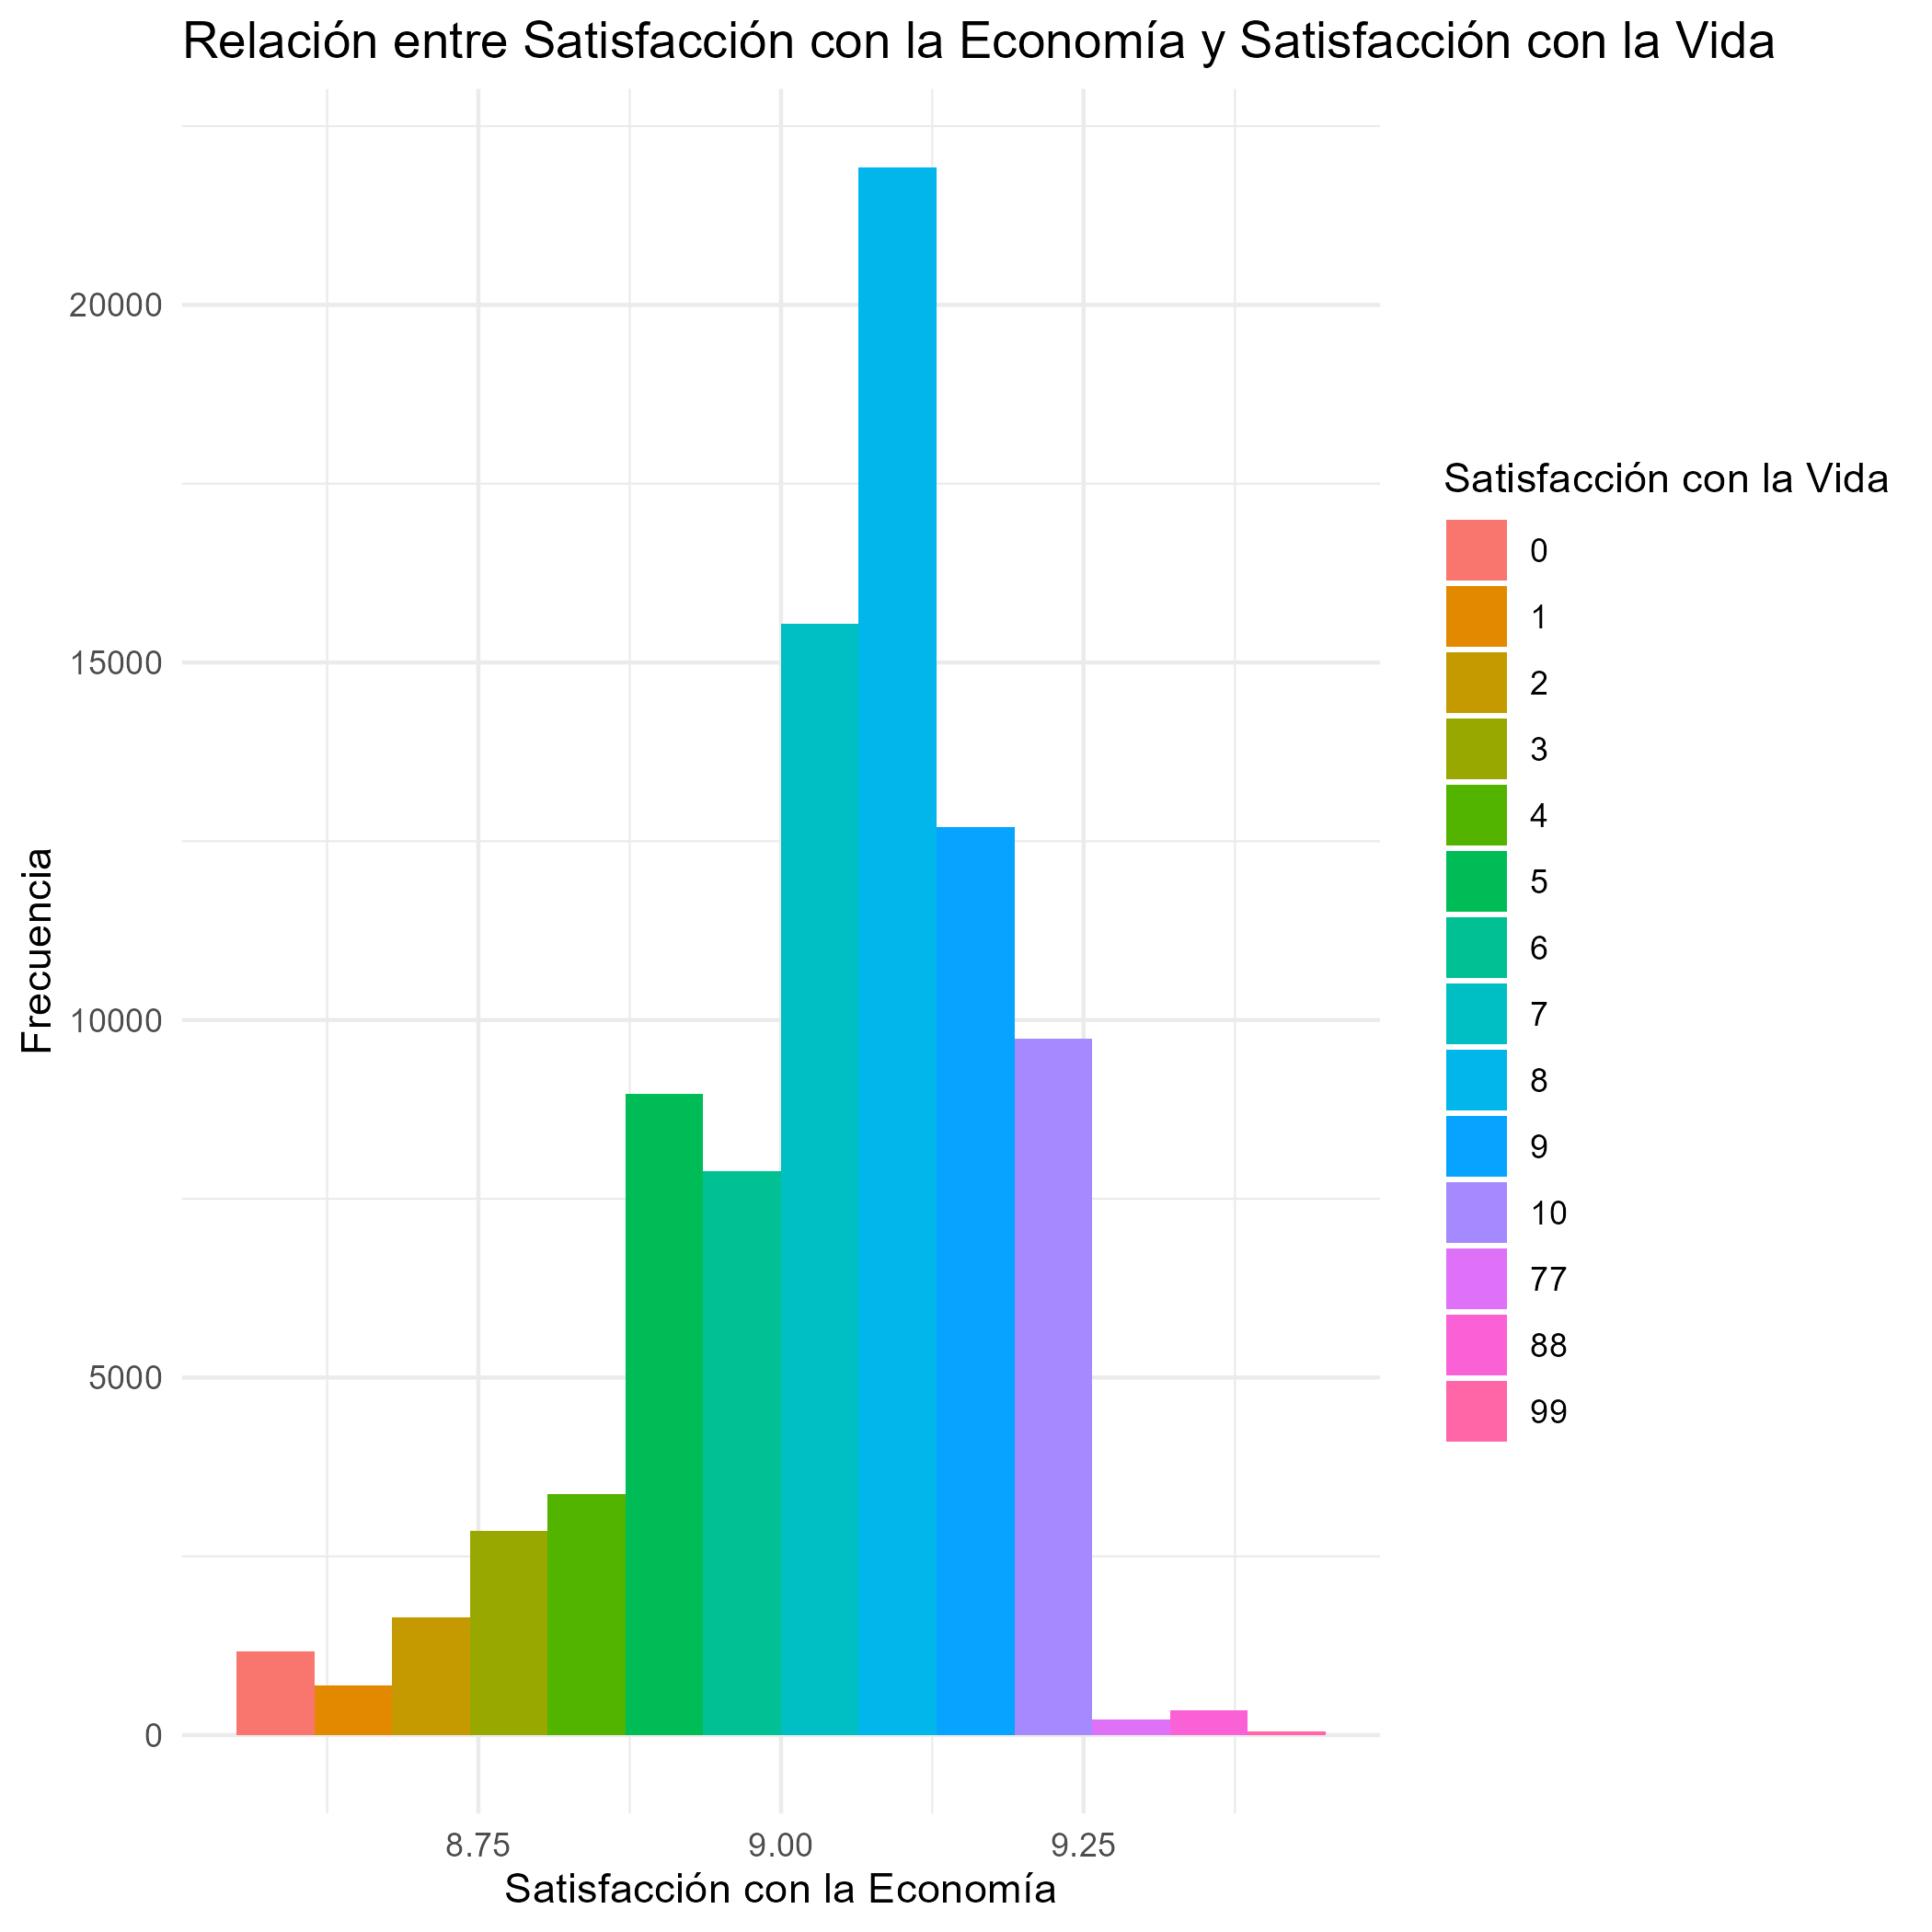
\includegraphics[width=\maxwidth]{relacion_satisfaccion_vida_economia} 

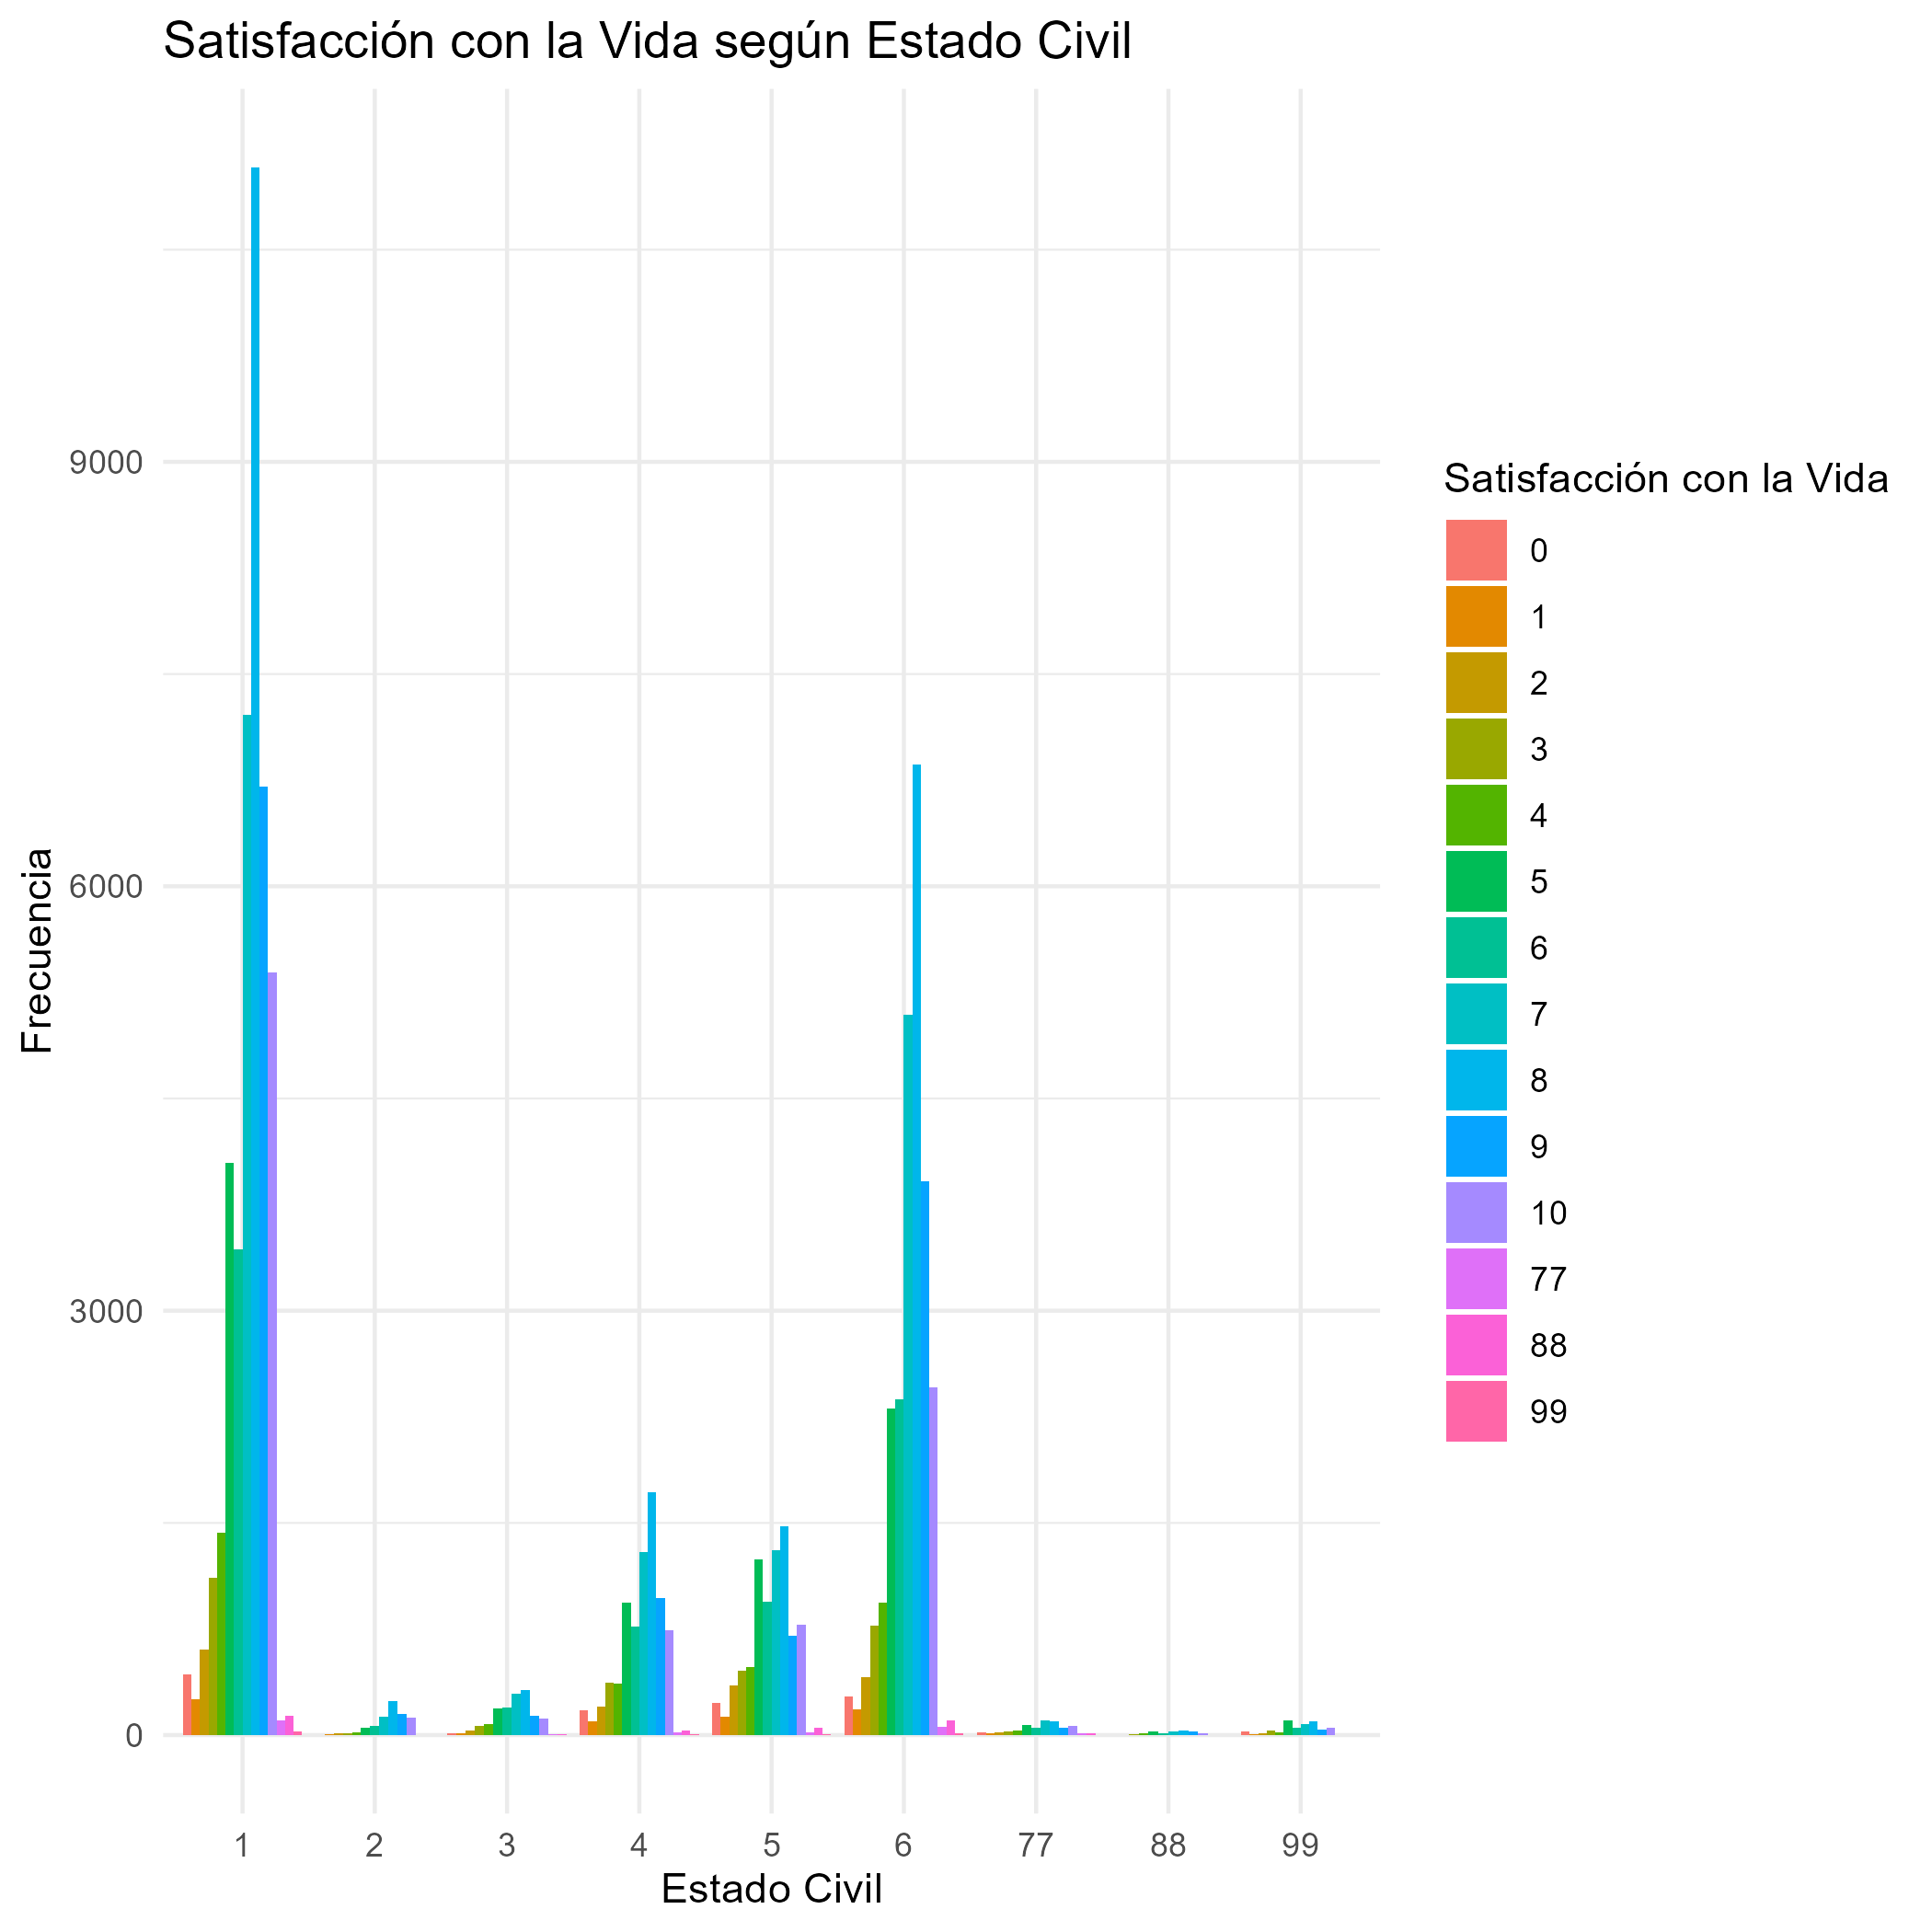
\includegraphics[width=\maxwidth]{satisfaccion_vida_estado_civil} 

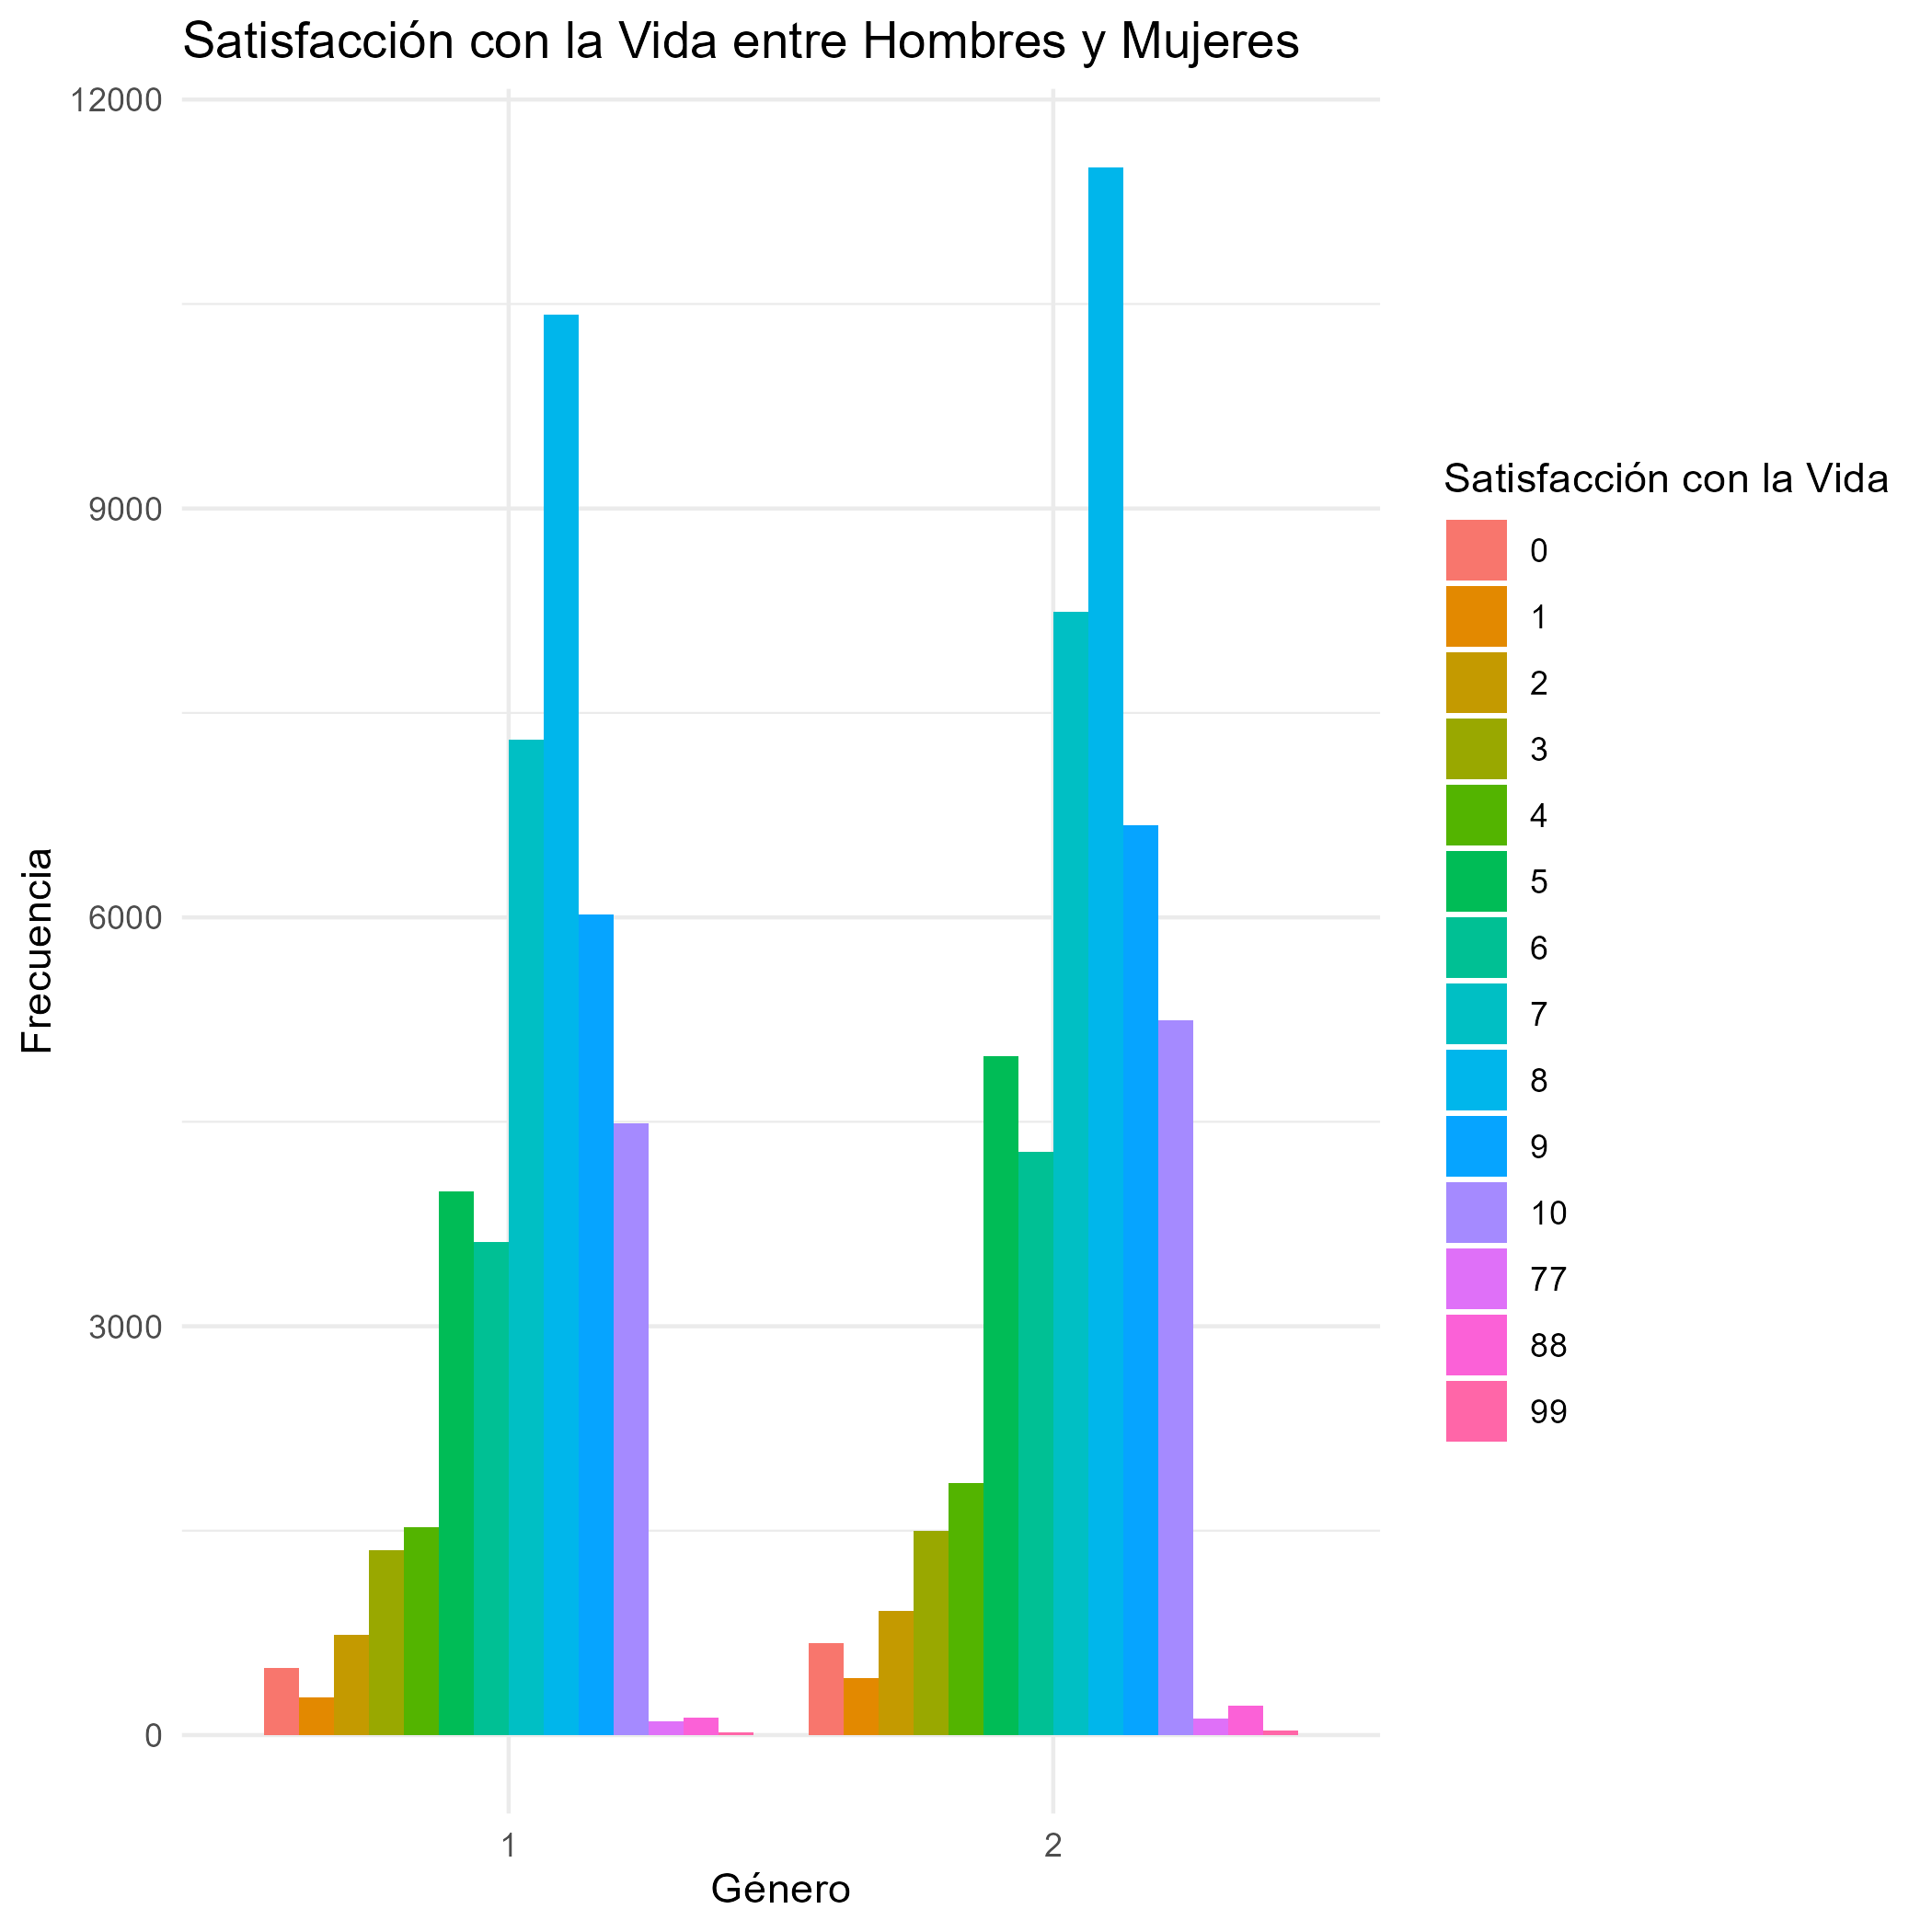
\includegraphics[width=\maxwidth]{satisfaccion_vida_genero} 

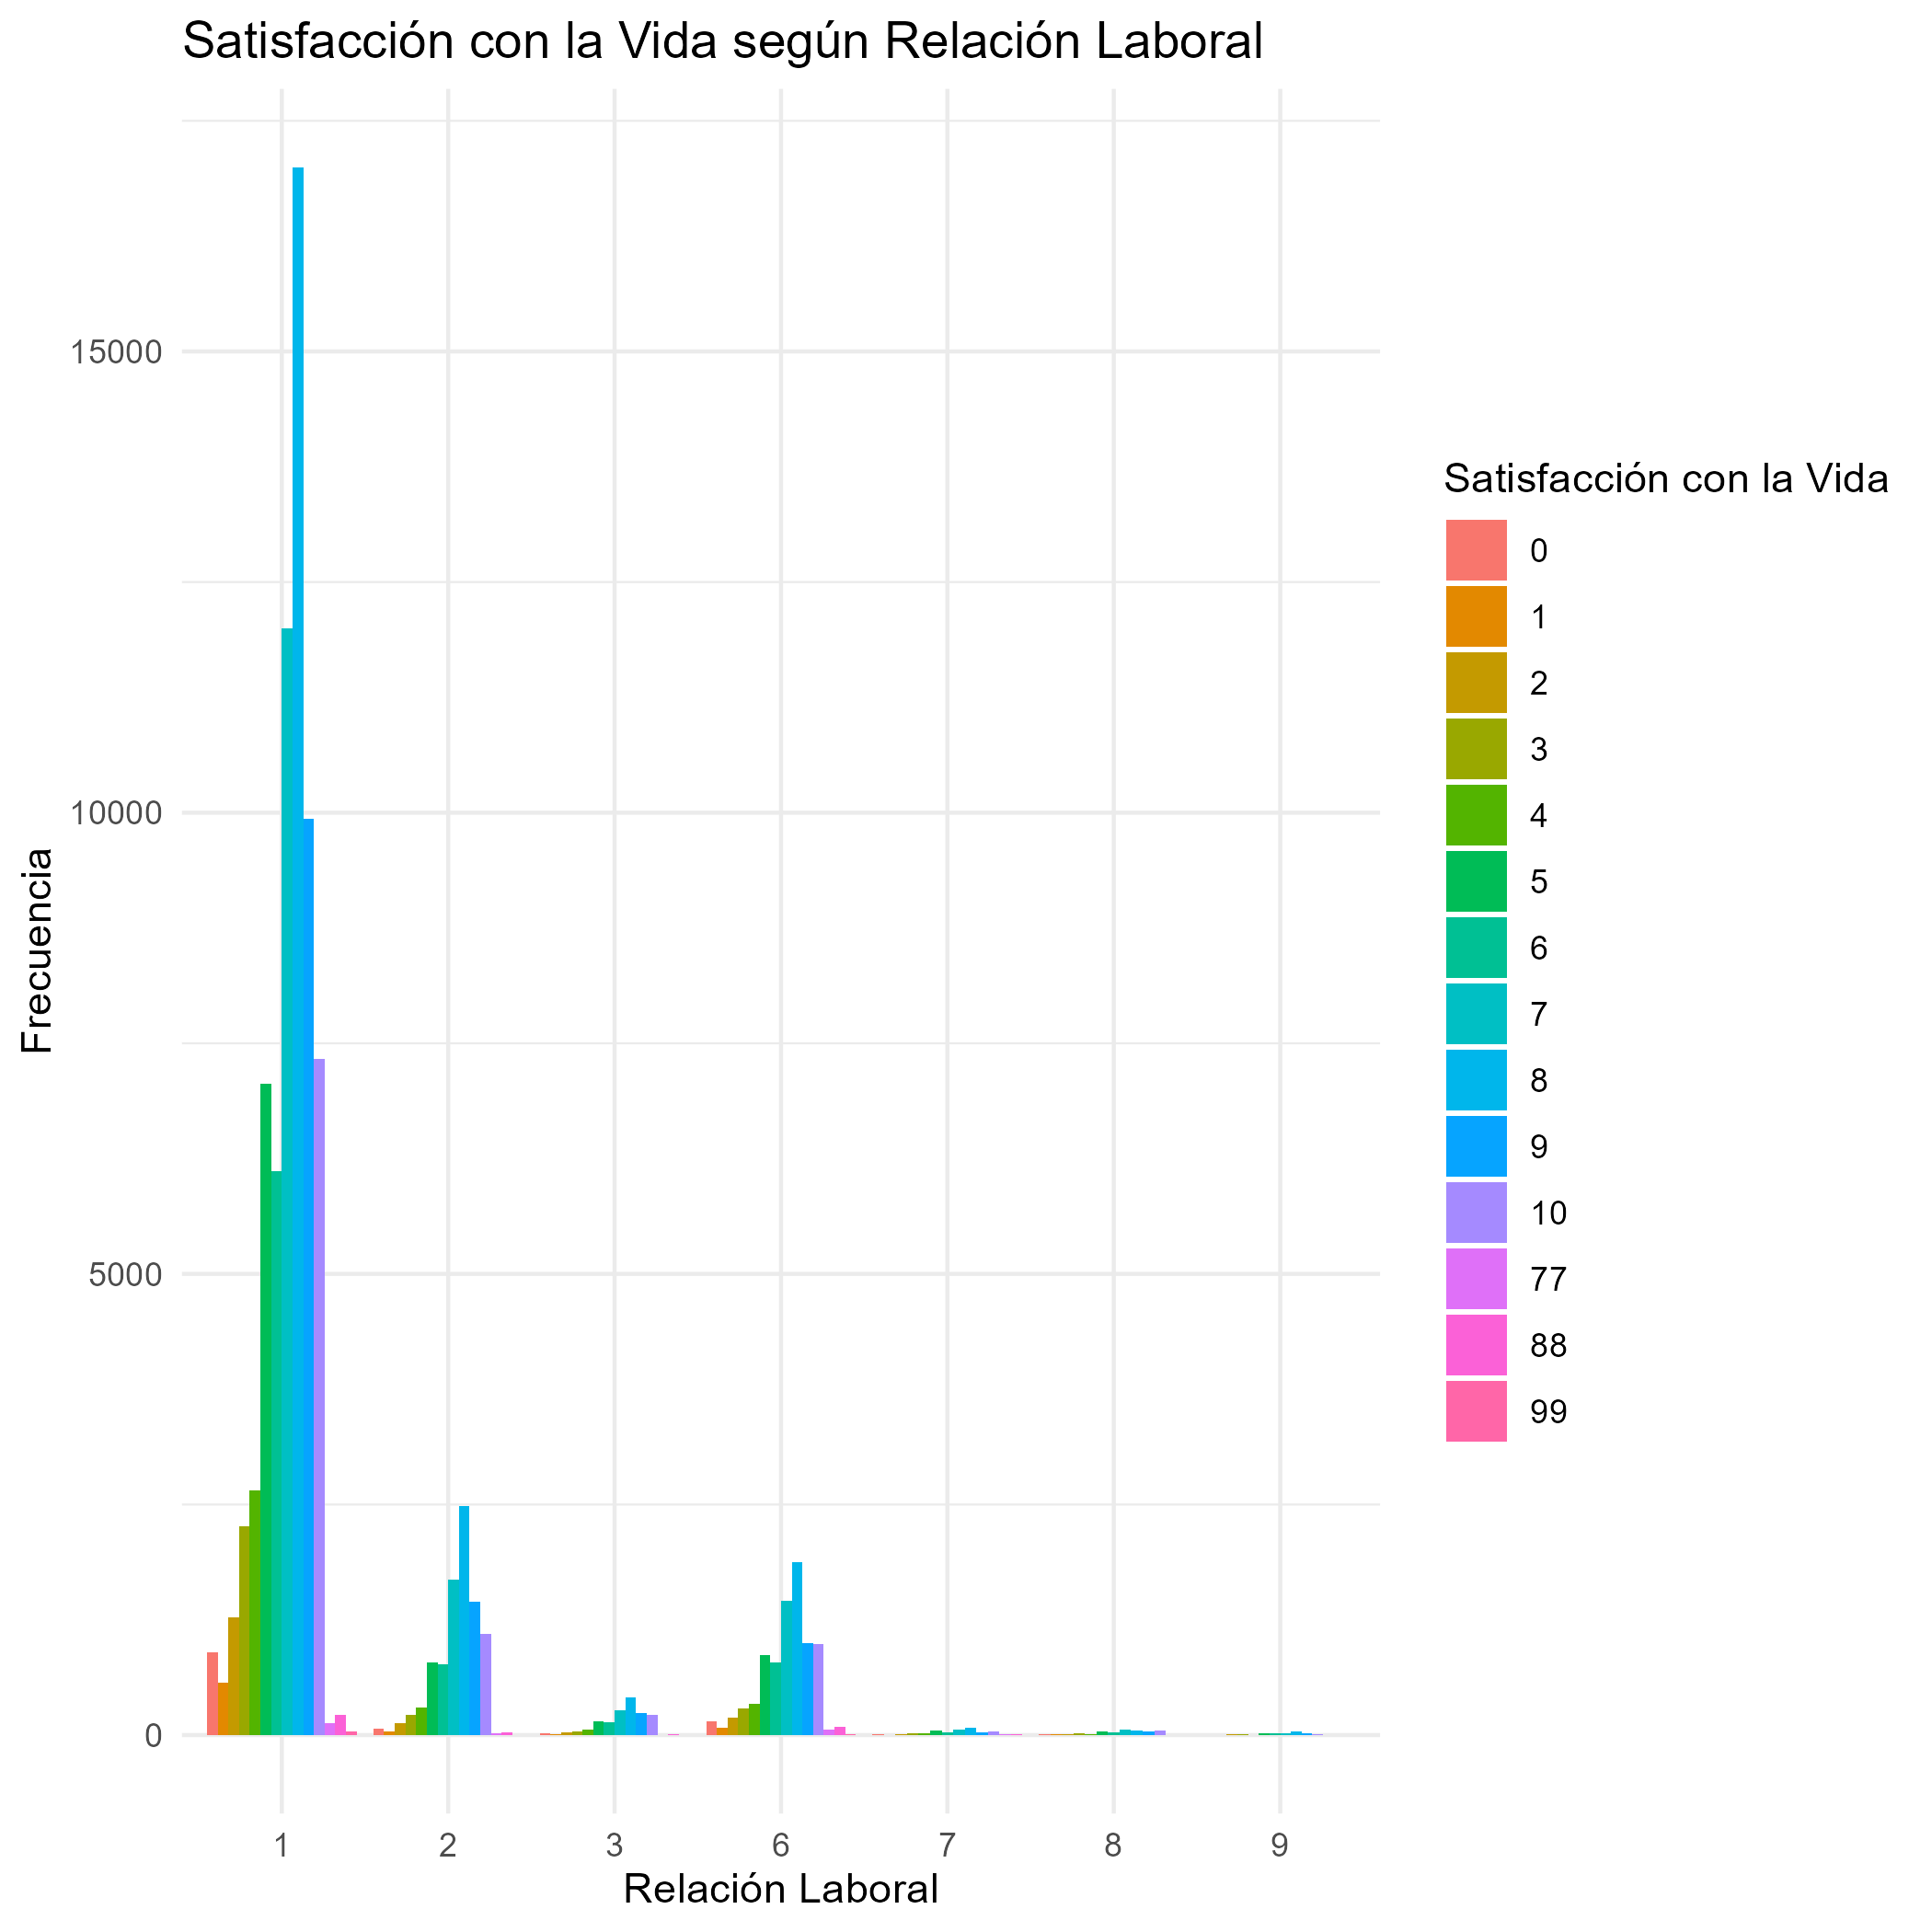
\includegraphics[width=\maxwidth]{satisfaccion_vida_relacion_laboral} 


\section{Explicaciones que combinen resultados de R (insertados mediante código) con texto con formato}

La media de la edad de los encuestados es \textbf{\emph{56.5660852}} años, con una desviación estándar de \textbf{\emph{74.9179991}} años. La tabla siguiente muestra un resumen de las estadísticas descriptivas.

\subsection{Tabla estadística descriptiva}

\begin{kframe}


{\ttfamily\noindent\itshape\color{messagecolor}{\#\# Rows: 1 Columns: 6\\\#\# -- Column specification --------------------------------------------------------\\\#\# Delimiter: "{},"{}\\\#\# dbl (6): Edad\_Media, Edad\_SD, Satisfaccion\_Vida\_Media, Satisfaccion\_Vida\_SD,...\\\#\# \\\#\# i Use `spec()` to retrieve the full column specification for this data.\\\#\# i Specify the column types or set `show\_col\_types = FALSE` to quiet this message.}}\end{kframe}\begin{table}

\caption{\label{tab:table_chunk}Tabla de Estadísticas Descriptivas}
\centering
\begin{tabular}[t]{r|r|r|r|r|r}
\hline
Edad\_Media & Edad\_SD & Satisfaccion\_Vida\_Media & Satisfaccion\_Vida\_SD & Felicidad\_Media & Felicidad\_SD\\
\hline
56.56609 & 74.918 & 8.131769 & 2.185627 & 8.357512 & 1.949245\\
\hline
\end{tabular}
\end{table}



\end{document}

